\documentclass[a4paper]{article}

\usepackage[utf8]{inputenc}
\usepackage[T1]{fontenc}
\usepackage{textcomp}
\usepackage{amsmath, amssymb}
\usepackage{array,multirow,graphicx}
\usepackage{float}
\usepackage{booktabs}
\usepackage{hyperref}
\usepackage{subcaption}
\usepackage{biblatex}
\addbibresource{report.bib}


% figure support
\usepackage{import}
\usepackage{xifthen}
\pdfminorversion=7
\usepackage{pdfpages}
\usepackage{transparent}
\newcommand{\incfig}[1]{%
	\def\svgwidth{\columnwidth}
	\import{./figures/}{#1.pdf_tex}
}

\pdfsuppresswarningpagegroup=1


\title{NPFL103 Information Retrieval: Assignment 2}
\date{\today}
\author{Andrew McIsaac}

\begin{document}
\maketitle

\section{Introduction}
This report explores using publicly available information retrieval frameworks
for retrieval on documents in both English and Czech. I use Elasticsearch, a
distributed, RESTful search engine. It is built on Apache Lucene, a Java library
which provides both indexing and search features. I explore and evaluate the
capabilities of Elasticsearch in terms of text analysis features, similarity
score weightings and measurements, and boosting of query terms. I also look at
a form of pseudo-relevance feedback based on significant terms.

\section{Index Construction}
Elasticsearch accepts JSON objects as inputs to be indexed. The documents can be
converted to python dictionaries and serialized to JSON by the Elasticsearch
python package. Each tag in every document is a separate field indexed by the
indexer, and the metafield \texttt{"\_id"}, used by Elasticsearch to differentiate
documents, is set to be the same as the \texttt{"docid"} field. For all
properties, the type is text so that they can be analyzed by the analyzer. The
analyzer is either language-specific, or a simple whitespace tokenizer for
\texttt{run-0}.

For creating the different indices I used various templates which provide the
language-specific settings, as well as other things which become useful in
experimentation, such as changing the similarity scoring method. Since this is
an experimental setup and I am not taking advantage of Elasticsearch's
distributed capabilities, I did not set up anything regarding security or
replication of data, and the number of shards was set to 1, as multiple shards
can make the way documents are scored be inconsistent, so that the retrieved 
score may not always be the correct one.

\section{Query Processing and Retrieval}

\section{Baseline Results}
With the constrained baseline results as specified in the assignment brief, my
system achieved a mean average precision (MAP) score of 0.0561 on the Czech
training topics, and a P$_{10}$ score of 0.060. The averaged 11-point
precision/recall graph is shown in Fig. \ref{fig:cs_train}. In all experiments,
only the \texttt{"text"} field was used for searching. Searching using different
fields in addition did not improve results on the training data.

For the English documents, the baseline MAP score was 0.0802, with a P$_{10}$
score of 0.128. The averaged 11-point precision/recall graph is shown in Fig.
\ref{fig:en_train}. In all experiments, the fields \texttt{\{"te", "dc", "dh",
		"ld", "cp",	"dl", "hd"\}} were used for search.

\begin{figure}[htpb]
	\centering
	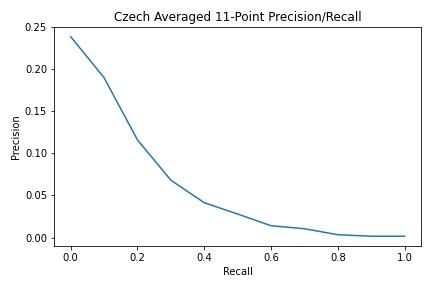
\includegraphics[width=0.8\textwidth]{plot_run-0_cs_precision_recall.jpg}
	\caption{Averaged 11-point Precision/Recall for Czech training data on run-0}
	\label{fig:cs_train}
\end{figure}

\begin{figure}[htpb]
	\centering
	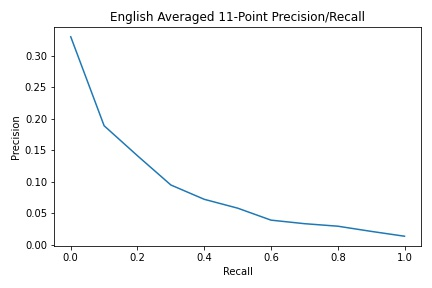
\includegraphics[width=0.8\textwidth]{plot_run-0_en_precision_recall.jpg}
	\caption{Averaged 11-point Precision/Recall for English training data on run-0}
	\label{fig:en_train}
\end{figure}

\section{Experiments}

\subsection{Text Analysis Functions}
\label{sec:text-analysis}
The built-in language analyzers for both Czech and English perform lowercasing,
stopword removal, and stemming on all indexed tokens. From the first assignment,
English documents performed best with these settings, while lemmatization
performed better than stemming in most cases for Czech. However, the built-in
Czech analyzer still seemed to work well with stemming in this instance. Default
settings for the analyzer used a 'standard' tokenizer based on the Unicode Text
Segmentation\footnote{\url{https://unicode.org/reports/tr29/}} algorithm. 

Further filters were available, such as fuzziness, which would search for tokens
which matched query terms with an edit distance of up to 2. This is particularly
useful for queries where a spelling error may have been made, for example, but
preliminary findings with these filters found no benefit to performance for
either English or Czech. This is probably because all queries are spelt
correctly, and terms are relatively short and are already subject to stemming
which reduces the likelihood of a token that is within the edit distance of the
query term being useful for the query.


\subsection{Similarity Scores}
\label{sec:similarity}
The default similarity score used by Elasticsearch is Okapi BM25 with $b=0.75$
and $k_1 = 1.2$. Since BM25 performed better than most other similarity
weightings for most people in Assignment 1, I did not experiment with any other
variant of tf-idf that has been explored previously. I did, however, briefly
explore the other similarities that come built-in with Elasticsearch
\footnote{\url{https://www.elastic.co/guide/en/elasticsearch/reference/current/index-modules-similarity.html\#_available_similarities}},
and used grid search to explore the best parameters for BM25.

\begin{table}[htpb]
    \centering
    \caption{Similarities MAP values for English}
    \label{tab:similarities}
    \begin{tabular}{c|c}
    Similarity & MAP \\
    \hline
    BM25 (default) & 0.3320 \\
    LM Jelinek Mercer & 0.3174 \\
    LM Dirichlet & 0.3232 \\
    DFR & 0.2957 \\
    DFI & 0.2742 \\
    IB & 0.3439
    \end{tabular}
\end{table}

The information-based model performs slightly better here than BM25, but when
tuned the BM25 model slightly outperforms IB (see Table \ref{tab:bm25}).

\begin{table}[htpb]
    \centering
    \caption{BM25 Hyperparameter Search English, optimizing for MAP.
    Best parameters are $b=0.5$, $k_1=1.8$}
    \label{tab:bm25}
    \begin{tabular}{|c|c|c|c|c|c|c|c|}
        \hline
     k1~\textbackslash~b & 0.3 & 0.4 & 0.5 & 0.6 & 0.7 & 0.8 & 0.9 \\
     \hline
     0.6 & 0.323 & 0.321 & 0.322 & 0.318 & 0.317 & 0.318 & 0.317 &
     0.8 & 0.328 & 0.342 & 0.322 & 0.324 & 0.322 & 0.322 & 0.323 &
     1.0 & 0.327 & 0.334 & 0.331 & 0.328 & 0.329 & 0.331 & 0.325 &
     1.2 & 0.332 & 0.339 & 0.340 & 0.338 & 0.335 & 0.331 & 0.325 &
     1.4 & 0.335 & 0.342 & 0.340 & 0.338 & 0.338 & 0.331 & 0.327 &
     1.6 & 0.338 & 0.345 & 0.342 & 0.340 & 0.336 & 0.329 & 0.330 &
     1.8 & 0.337 & 0.344 & \textbf{0.345} & 0.341 & 0.338 & 0.330 & 0.328 &
     2.0 & 0.335 & 0.341 & 0.343 & 0.340 & 0.339 & 0.329 & 0.325 &
     \hline
    \end{tabular}
\end{table}

A similar table produced for Czech (not shown here) gives optimal parameters
for $b$ and $k_1$ as 0.3 and 0.6 respectively. The MAP is 0.3362. The
corresponding $p_{10}$ value for Czech is 0.348, while for English the best
Hyperparameters give a MAP of 0.345 and a $p_{10}$ of 0.428.

\subsection{Query Boosting}
\label{sec:boosting}

I also experimented with boosting document scores when the exact query phrase
was present in the document. It seems probable that these documents would be
highly relevant to the query, and so should have their score boosted in favour
of those that maybe have a term occur more frequently but in a different context
and so is less relevant. However, I found that there was no benefit for English,
and while the MAP score for Czech does improve, the improvement is fairly small.
See Table \ref{tab:boosting}. The best result for Czech is 0.3443 MAP and 0.344
$P_{10}$, with a boost of 0.5.

\begin{table}[htpb]
    \centering
    \caption{Boosting of Exact Query Phrase Matches}
    \label{tab:boosting}
    \begin{tabular}{cc|cc}
    & Boost & MAP & P$_{10}$ &
    \hline
    \parbox[t]{2mm}{\multirow{4}{*}{\rotatebox[origin=c]{90}{English}}} 
    & 3 & 0.3332 & 0.392 &
    & 2 & 0.3339 & 0.388 &
    & 1 & 0.3367 & 0.396 &
    & 0.5 & 0.3444 & 0.408 &
    \hline
    \parbox[t]{2mm}{\multirow{4}{*}{\rotatebox[origin=c]{90}{Czech}}} 
    & 3 & 0.3405 & 0.340 &
    & 2 & 0.3409 & 0.340 &
    & 1 & 0.3420 & 0.340 &
    & 0.5 & 0.3443 & 0.344 &
    \end{tabular}
\end{table}

\subsection{Pseudo-Relevance / Query Expansion}
Finally, I used a form of pseudo-relevance feedback to expand the queries with
significant terms from retrieved documents\footnote{\url{https://www.elastic.co/guide/en/elasticsearch/reference/current/search-aggregations-bucket-significanttext-aggregation.html}}.
This works by extracting terms that are in a significantly higher portion of the
returned documents than the total number of indexed documents, then adding some
of these terms to the query and re-querying with these expanded terms to find
more relevant documents that don't contain exactly the words that were used in
the query.

For example, the query "Renewable Energy Sources" has the following significant
terms (in their tokenized, stemmed forms): geotherm, biomass, solar. Clearly
documents that contain these terms and nothing from the original query may still
be relevant to the original query, as they are all examples of renewable energy
sources. 

This technique can lead to query drift however. With the query "Euro Inflation",
"yen" is one of the significant terms that comes up from its relevant documents,
which could be because the documents talk about the relative prices of multiple
currencies on foreign exchange markets, and so both the Euro and the Yen are
mentioned. But articles that focus on the Yen will not be relevant to the
original query.

I experimented with different numbers of retrieved documents from which to
extract these significant terms, and found that the best results were when just
the most relevant 10 were used, for both Czech and English. This may be because
some of the documents outside the top few were not in fact relevant and would
skew the results towards less related significant terms. The MAP for Czech was
0.3595, with a $p_{10}$ of 0.348, while for English the MAP was 0.3502 and the
$p_{10}$ was 0.416.

\section{Run-1 Results}

The best results for Czech were obtained using the standard analyzer for Czech,
boosted exact query phrase matches with a boost of 0.5, BM25 similarity with
$b=0.3$ and $k_1=0.6$, and using pseudo-relevance feedback to expand queries
based on the top 10 most relevant documents. The averaged 11-point
precision/recall graph is shown in Fig. \ref{fig:cs_train_run_1}. The MAP was
0.3595 and the $P_{10}$ was 0.348.


\begin{figure}[htpb]
	\centering
	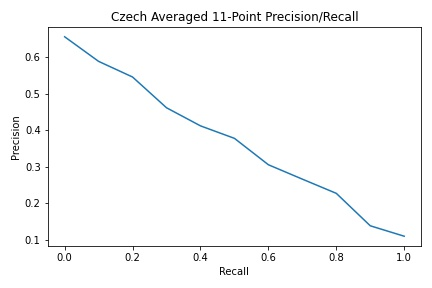
\includegraphics[width=0.8\textwidth]{plot_run-1_cs_precision_recall.jpg}
	\caption{Averaged 11-point Precision/Recall for Czech training data on run-1}
	\label{fig:cs_train_run_1}
\end{figure}

The best results for English were obtained using the standard analyzer for
English, standard queries with no boost, BM25 similarity iwth $b=0.5$ and
$k_1=1.8$, and using pseudo-relevance feedback to expand queries based on the
top 10 most relevant documents. The averaged 11-point precision/recall graph is
shown in Fig. \ref{fig:en_train_run_1}. The MAP was 0.3502 and the $P_{10}$ was
0.416.

\begin{figure}[htpb]
	\centering
	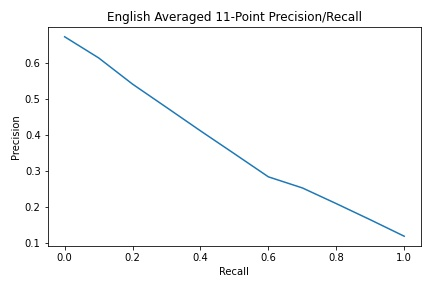
\includegraphics[width=0.8\textwidth]{plot_run-1_en_precision_recall.jpg}
	\caption{Averaged 11-point Precision/Recall for English training data on run-1}
	\label{fig:en_train_run_1}
\end{figure}

\section{Conclusion}
In this report, I evaluated Elasticsearch as a tool for state-of-the-art
information retrieval. I explored some different methods for text analysis
supported by Elasticsearch, and looked in detail at the options for scoring
and query modification to improve the precision and relevance of retrieved
documents for queries. The default settings worked pretty well, especially for
text analysis, where no additional filters I tried improved the relevance of
retrieved documents in any of the experiments. Slight improvements on the
training documents were reported with tweaked BM25 parameters, and further
small improvements were made with modifications to queries to boost more
relevant documents up the rankings, and to find new documents that are relevant,
but were previously undiscovered.

Interestingly, both English and Czech had very similar results in most
experiments, with the best MAP scores around 0.35. The differences in the
languages did not affect the ability to retrieve documents. Compared to
the first assignment, this was a surprise, where often the performance of the
best-performing system would be significantly different in one language than the
other. This may be because of better tuning of language-specific features in
the standard analyzers for each language. A fully-tested and robust codebase
in Elasticsearch may also be a factor in this extra consistency.

My results were much better than in assignment 1. I think a large part of this
was due to BM25. I did not use it in assignment 1, and systems that did use it
generally performed better, and it is shown again here. It is interesting that
stemming did not cause any problems for the Czech language in this case. Perhaps
the stemming algorithm used differed to be more reflective of the language,
although I do not speak Czech so cannot comment too much on the details.

\printbibliography

\newpage

\appendix

\section{Set Up and Running Experiments}

Make sure all requirements are installed, including an active Elasticsearch
cluster. Docker is recommended, but alternative methods should also work, as
long as it is exposed at \texttt{localhost:9200}:
\begin{verbatim}
pip install -r requirements.txt
docker network create elastic
docker pull docker.elastic.co/elasticsearch/elasticsearch:7.16.2
docker run --name es01-ir --net elastic
    -p 127.0.0.1:9200:9200 -p 127.0.0.1:9300:9300
    -e "discovery.type=single-node"
    docker.elastic.co/elasticsearch/elasticsearch:7.16.2
\end{verbatim}

To run experiments run the following commands, replacing the LANGUAGE
and QUERIES environment variables where appropriate. The program must
be run from the parent directory of the documents.
\begin{verbatim}
export LANGUAGE="en"
export LANGUAGE="cs"
export QUERIES="train"
export QUERIES="test"
python run-0.py
python run-1.py
\end{verbatim}

\end{document}
